\chapter{Chef Server}

The Chef Server acts as a hub for configuration data. The server stores cookbooks, the policies that are applied to nodes, and metadata that describes each registered node that is being managed by the chef-client. Nodes use the chef-client to ask the server for configuration details, such as recipes, templates, and file distributions. The chef-client then does as much of the configuration work as possible on the nodes themselves (and not on the server). This scalable approach distributes the configuration effort throughout the organization.

The diagram~\ref{fig:overview_chef_draft} shows the relationships between the various elements of Chef, including the nodes, the server, and the workstations. These elements work together to provide the chef-client the information and instruction that it needs so that it can do its job.

\begin{figure}[ht!]
  \center{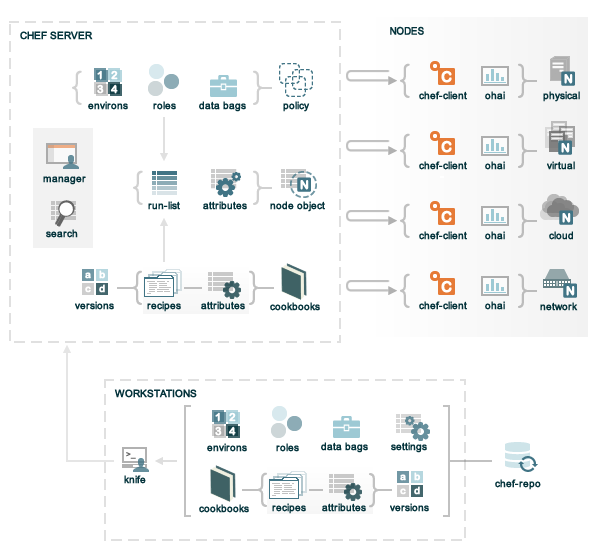
\includegraphics[width=1\textwidth]{overview_chef_draft}}
  \caption{Chef Infrastructure}
  \label{fig:overview_chef_draft}
\end{figure}

We will learn Chef Server by practical examples in this chapter.

\section{Installation}
\label{sec:server-installation}

Exists several ways to install own Chef Server:

\begin{itemize}
  \item Go to \href{http://www.getchef.com/chef/install/}{www.getchef.com/chef/install}, select the operating system, version, and architecture of the server and install the downloaded package on it. After installation you can configure server by command <<sudo chef-server-ctl reconfigure>>
  \item Use Chef Solo to install Chef Server
\end{itemize}

Of course, I prefer to use Chef Solo to install and configure Chef Server. Chef Solo will help us quickly deploy Chef Server on a new server, if something happens with it (crash file system of server, etc.). Do not forget to make a backups of Chef Server (because compared with Chef Solo, Chef Server will be the point of failure in your configuration management system).

Let's create our folder, which will contain all our Chef kitchen:

\begin{lstlisting}[language=Bash,label=lst:my-server-cloud-installation1]
$ mkdir my-server-cloud
$ cd my-server-cloud
$ cat Gemfile
source "https://rubygems.org"

gem 'chef'
gem 'berkshelf'
$ bundle
$ git clone https://github.com/opscode/chef-repo.git .
# or you can use "knife solo init .", if you will install knife-solo
\end{lstlisting}

To install and configure Chef Server exists cookbook \href{https://supermarket.getchef.com/cookbooks/chef-server}{chef-server}. Let's add this cookbook in Berkshelf:

\begin{lstlisting}[label=lst:my-server-cloud-installation2,title=my-server-cloud/Berkshelf]
source "http://api.berkshelf.com"

cookbook 'chef-server'
\end{lstlisting}

After running the command <<berks install>> this cookbook will be installed with dependencies.

\begin{lstlisting}[language=Bash,label=lst:my-server-cloud-installation3]
$ berks install
Installing chef-server (2.0.1) from site: 'http://cookbooks.opscode.com/api/v1/cookbooks'
$ berks install --path cookbooks
Using chef-server (2.0.1)
\end{lstlisting}

Now we should configure a Chef Solo node for our Chef Server. From chapter <<\ref{sec:solo-node}~\nameref{sec:solo-node}>> you should know how to define node.

\begin{lstlisting}[language=JSON,label=lst:my-server-cloud-installation4,title=my-server-cloud/nodes/chef-server.example.com.json]
{
  "fqdn": "10.33.33.33",
  "chef-server": {
    "api_fqdn": "10.33.33.33",
    "version": "latest",
    "configuration": {
      "notification_email": "notify@example.com",
      "chef-server-webui": {
        "enable": true
      }
    }
  },
  "run_list": [
    "recipe[chef-server]"
  ]
}
\end{lstlisting}

By \lstinline!configuration! key you can change settings for Chef Server. All available setting, which can be redefined, you can find \href{https://github.com/opscode/omnibus-chef-server/blob/master/files/chef-server-cookbooks/chef-server/attributes/default.rb}{here}. Our Chef Server by default takes your systems \href{http://en.wikipedia.org/wiki/Fully\_qualified\_domain\_name}{FQDN} as Chef Server url, what is why I set <<fqdn>> in node IP 10.33.33.33, which will set to my server by Vagrant.

First, we should generate Vagrantfile:

\begin{lstlisting}[language=Bash,label=lst:my-server-cloud-installation5]
$ vagrant init precise64
A `Vagrantfile` has been placed in this directory. You are now
ready to `vagrant up` your first virtual environment! Please read
the comments in the Vagrantfile as well as documentation on
`vagrantup.com` for more information on using Vagrant.
\end{lstlisting}

Next we need modeling a cluster of machines by Vagrant. Right now we need only chef server. Let's modify Vagrantfile:

\begin{lstlisting}[label=lst:my-server-cloud-installation6,title=my-server-cloud/Vagrantfile]
# -*- mode: ruby -*-
# vi: set ft=ruby :

require 'chef'
require 'json'

Chef::Config.from_file(File.join(File.dirname(__FILE__), '.chef', 'knife.rb'))

chef_server_json = JSON.parse(Pathname(__FILE__).dirname.join('nodes', 'chef-server.example.com.json').read)

# Vagrantfile API/syntax version. Don't touch unless you know what you're doing!
VAGRANTFILE_API_VERSION = "2"

Vagrant.configure(VAGRANTFILE_API_VERSION) do |config|

  config.vm.define :chef_server do |chef_server|
    chef_server.vm.box = "precise64"
    chef_server.vm.network "private_network", ip: "10.33.33.33"

    chef_server.vm.provision :chef_solo do |chef|
      chef.cookbooks_path = Chef::Config[:cookbook_path]
      chef.roles_path = Chef::Config[:role_path]
      chef.data_bags_path = Chef::Config[:data_bag_path]
      chef.environments_path = Chef::Config[:environment_path]

      chef.run_list = chef_server_json.delete('run_list')
      chef.json = chef_server_json
    end
  end

end
\end{lstlisting}

You should have installed chef gem inside vagrant, as we did in chapter <<\ref{sec:solo-vagrant}~\nameref{sec:solo-vagrant}>> and install/update Chef Client inside server by command <<knife solo prepare>>.

\begin{lstlisting}[language=Bash,label=lst:my-server-cloud-installation7]
$ vagrant provision
[chef_server] Running provisioner: chef_solo...
Generating chef JSON and uploading...
Running chef-solo...
stdin: is not a tty
INFO: Forking chef instance to converge...
INFO: *** Chef 11.8.2 ***
INFO: Chef-client pid: 1831
INFO: Setting the run_list to ["recipe[chef-server]"] from JSON
INFO: Run List is [recipe[chef-server]]
INFO: Run List expands to [chef-server]
...
\end{lstlisting}

We can check Chef Server web interface by \href{https://10.33.33.33}{https://10.33.33.33} and info about libraries version by \href{https://10.33.33.33/version}{https://10.33.33.33/version} url. It should looks like on figure~\ref{fig:chef-server-versions}.

\begin{figure}[ht!]
  \center{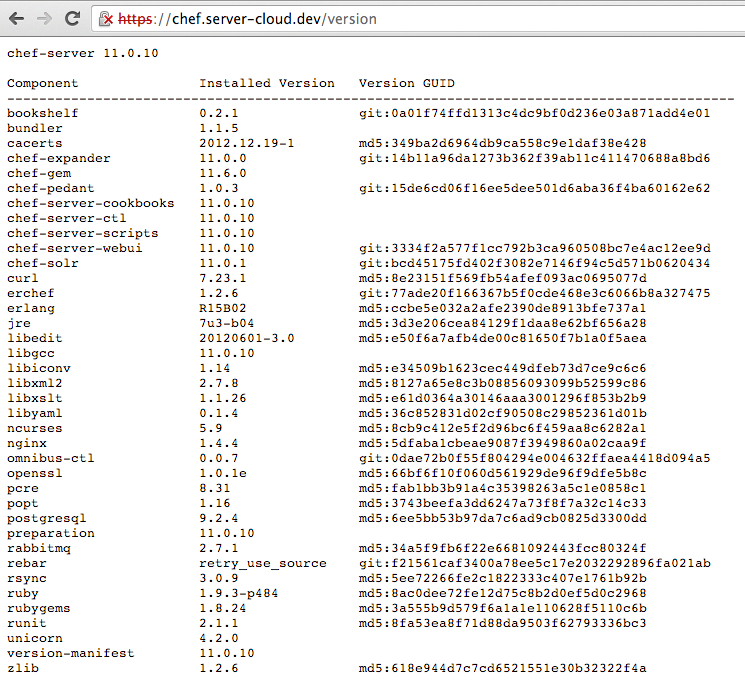
\includegraphics[width=1\textwidth]{chef_server_versions}}
  \caption{Chef Server Versions}
  \label{fig:chef-server-versions}
\end{figure}

I most cases web interface give information about your cloud, which you can get from knife tool. What is why generally it disabled by attribute <<chef-server-webui.enable = false>>.

Next we should configure our knife to work with this Chef Server.

\section{Attributes}\label{sec:server-attributes}

An attribute is a specific detail about a node. Attributes are used by the chef-client to understand:

\begin{itemize}
  \item The current state of the node
  \item What the state of the node was at the end of the previous chef-client run
  \item What the state of the node should be at the end of the current chef-client run
\end{itemize}

As you read from previous sections of book, attributes can be defined in node, roles and environments, but it's also can be defined by cookbooks.

\subsection{Attribute Types}

Attribute types can be any of the following:

\begin{itemize}
  \item \textbf{default} - attribute is automatically reset at the start of every chef-client run and has the lowest attribute precedence
  \item \textbf{force\_default} - attribute is used to ensure that an attribute defined in a cookbook (by an attribute file or by a recipe) takes precedence over a default attribute set by a role or an environment
  \item \textbf{normal} - attribute is a setting that persists on the target system and is never reset during a chef-client run. A normal attribute has a higher attribute precedence than a default attribute
  \item \textbf{override} - attribute is automatically reset at the start of every chef-client run and has a higher attribute precedence than default, force\_default, and normal attributes. An override attribute is most often specified in a recipe, but can be specified in an attribute file, for a role, and/or for an environment
  \item \textbf{force\_override} - attribute is used to ensure that an attribute defined in a cookbook (by an attribute file or by a recipe) takes precedence over an override attribute set by a role or an environment
  \item \textbf{automatic} - attribute contains data that is identified by Ohai at the beginning of every chef-client run. An automatic attribute cannot be modified and always has the highest attribute precedence
\end{itemize}

At the beginning of a chef-client run, all default, override, and automatic attributes are reset. The chef-client rebuilds them using data collected by Ohai at the beginning of the chef-client run and by attributes that are defined in cookbooks, roles, and environments. Normal attributes are never reset. All attributes are then merged and applied to the node according to attribute precedence. At the conclusion of the chef-client run, all default, override, and automatic attributes disappear, leaving only a collection of normal attributes that will persist until the next chef-client run.

\subsection{Automatic (Ohai)}

An automatic attribute is a specific detail about a node, such as an IP address, a host name, a list of loaded kernel modules, and so on. Automatic attributes are detected by Ohai and are then used by the chef-client to ensure that these attribute are handled properly during every chef-client run. The most commonly accessed automatic attributes are:

\begin{itemize}
  \item \textbf{node['platform']} - the platform on which a node is running. This attribute helps determine which providers will be used
  \item \textbf{node['platform\_version']} - the version of the platform. This attribute helps determine which providers will be used
  \item \textbf{node['ipaddress']} - the IP address for a node. If the node has a default route, this is the IPV4 address for the interface. If the node does not have a default route, the value for this attribute should be nil. The IP address for default route is the recommended default value
  \item \textbf{node['macaddress']} - the MAC address for a node, determined by the same interface that detects the <<node['ipaddress']>>
  \item \textbf{node['fqdn']} - the fully qualified domain name for a node. This is used as the name of a node unless otherwise set
  \item \textbf{node['hostname']} - the host name for the nod
  \item \textbf{node['domain']} - the domain for the node
  \item \textbf{node['recipes']} - a list of recipes associated with a node (and part of that node’s run-list)
  \item \textbf{node['roles']} - a list of roles associated with a node (and part of that node’s run-list)
\end{itemize}

The list of automatic attributes that are collected by Ohai at the start of each chef-client run vary from organization to organization, and will often vary between the various server types being configured and the platforms on which those servers are run. All attributes collected by Ohai are unmodifiable by the chef-client.

\subsection{Attribute Precedence}

Attribute types can be any of the following:

\begin{enumerate}
  \item A \textbf{default} attribute located in a cookbook attribute file
  \item A \textbf{default} attribute located in a recipe
  \item A \textbf{default} attribute located in an environment
  \item A \textbf{default} attribute located in role
  \item A \textbf{force\_default} attribute located in a cookbook attribute file
  \item A \textbf{force\_default} attribute located in a recipe
  \item A \textbf{normal} attribute located in a cookbook attribute file
  \item A \textbf{normal} attribute located in a recipe
  \item An \textbf{override} attribute located in a cookbook attribute file
  \item An \textbf{override} attribute located in a recipe
  \item An \textbf{override} attribute located in a role
  \item An \textbf{override} attribute located in an environment
  \item A \textbf{force\_override} attribute located in a cookbook attribute file
  \item A \textbf{force\_override} attribute located in a recipe
  \item An \textbf{automatic} attribute identified by Ohai at the start of the chef-client run
\end{enumerate}

where the last attribute in the list is the one that is applied to the node.

Attribute precedence, viewed from the same perspective as the overview diagram~\ref{fig:overview_chef_attributes_precedence}, where the numbers in the diagram match the order of attribute precedence:

\begin{figure}[ht!]
  \center{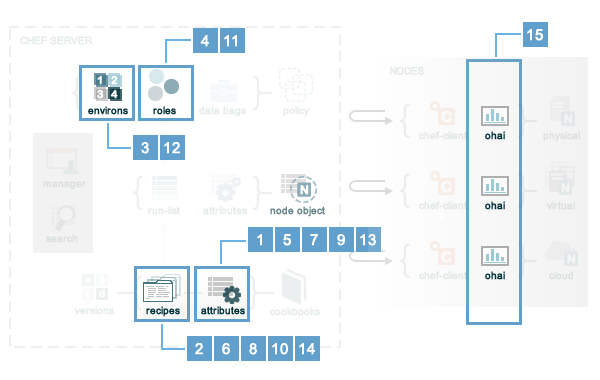
\includegraphics[width=1\textwidth]{overview_chef_attributes_precedence}}
  \caption{Attribute precedence}
  \label{fig:overview_chef_attributes_precedence}
\end{figure}

Attribute precedence~\ref{fig:overview_chef_attributes_table}, when viewed as a table:

\begin{figure}[ht!]
  \center{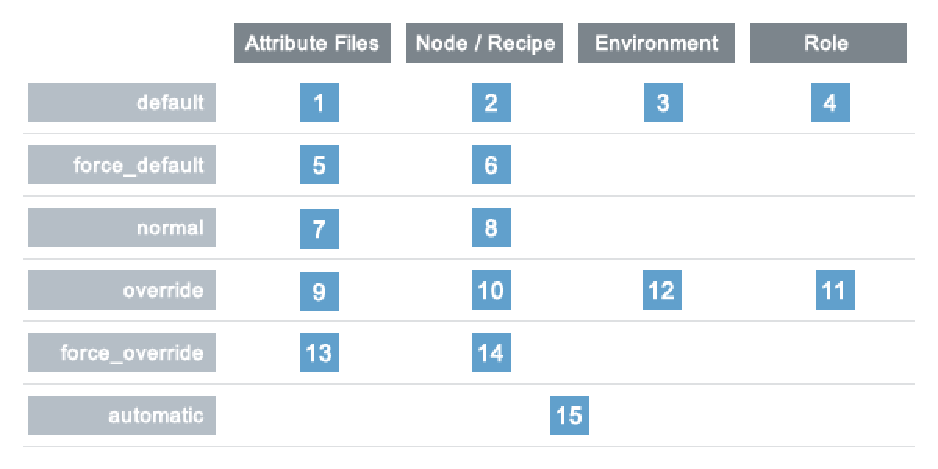
\includegraphics[width=1\textwidth]{overview_chef_attributes_table}}
  \caption{Attribute precedence}
  \label{fig:overview_chef_attributes_table}
\end{figure}
